%============================================================
% BAB 4 — EKSPERIMEN DAN ANALISIS
%============================================================
\chapter{EKSPERIMEN DAN ANALISIS}

Uraian pada bab ini meliputi parameter eksperimen, karakteristik data, skenario
ujicoba, tempat dan waktu eksperimen, spesifikasi peralatan ujicoba, cara penafsiran
dan penyimpulan hasil proyek akhir. Untuk proyek akhir yang menggunakan metode
kualitatif, dapat dijelaskan pendekatan yang digunakan, proses pengumpulan dan analisis
informasi, proses penafsiran, dan penyimpulan hasil proyek akhir. Analisis hasil
eksperimen seharusnya dihubungkan kembali dengan permasalahan.

\section{PARAMETER EKSPERIMEN}

Disini penulis dapat membahas parameter eksperimen lebih terperinci. Deskripsi
pembahasan seharusnya singkat, padat, dan jelas sehingga membuat pembaca memahami
maksud penulis yang tertuang dalam tulisan. Dalam eksperimen ini menggunakan persamaan
sebagai berikut:

\begin{equation}
  y = mx + c
  \label{eq:linear}
\end{equation}
\begin{equation}
  \frac{y - y_1}{x - x_1} = \frac{y_2 - y_1}{x_2 - x_1}
  \label{eq:gradien}
\end{equation}

Selain itu, dalam eksperimen ini juga menggunakan persamaan sebagai berikut untuk
formulasi perbandingan hasil pengukuran dengan perhitungan:

\begin{equation}
  v = v_0 + at
  \label{eq:glbb1}
\end{equation}
\begin{equation}
  s = v_0 t + \frac{1}{2}at^2
  \label{eq:glbb2}
\end{equation}
\begin{equation}
  v^2 = v_0^2 + 2as
  \label{eq:glbb3}
\end{equation}

\section{KARAKTERISTIK DATA}

Disini penulis dapat membahas karakteristik data lebih terperinci. Akan lebih baik jika
penulis dapat memberikan alasan terhadap penggunaan data yang mempunyai karakteristik
seperti itu. Deskripsi pembahasan seharusnya singkat, padat, dan jelas sehingga membuat
pembaca memahami maksud penulis yang tertuang dalam tulisan.

\section{TEMPAT UJICOBA}

Disini penulis dapat membahas tempat pelaksanaan ujicoba lebih terperinci. Deskripsi
pembahasan seharusnya singkat, padat, dan jelas sehingga membuat pembaca memahami
maksud penulis yang tertuang dalam tulisan.

\section{WAKTU UJICOBA}

Disini penulis dapat membahas waktu pelaksanaan ujicoba pada penelitian lebih detail.
Deskripsi pembahasan seharusnya singkat, padat, dan jelas sehingga membuat pembaca
memahami maksud penulis terkait dengan waktu yang digunakan untuk ujicoba pada
penelitian.

\section{SPESIFIKASI PERALATAN UJICOBA}

Disini penulis dapat membahas spesifikasi peralatan lebih terperinci. Peralatan dapat
berupa perangkat keras, perangkat lunak, piranti elektronik, \textit{gadget}, dan
lain-lain yang berfungsi sebagai alat yang dipakai untuk percobaan. Deskripsi
pembahasan seharusnya singkat, padat, dan jelas sehingga membuat pembaca memahami
maksud penulis yang tertuang dalam tulisan.

\section{HASIL EKSPERIMEN}

Disini penulis dapat membahas hasil eksperimen lebih terperinci. Deskripsi pembahasan
seharusnya singkat, padat, dan jelas sehingga membuat pembaca memahami maksud penulis
yang tertuang dalam tulisan.

% ── Tabel-tabel hasil eksperimen ─────────────────────────────
\begin{table}[H]
  \centering
  \caption{Contoh tabel hasil eksperimen 1}
  \label{tab:hasil1}
  \begin{tblr}{colspec={c c c c}}
    Kolom 1 & Kolom 2 & Kolom 3 & Kolom 4 \\
    & & & \\
    & & & \\
  \end{tblr}
\end{table}

\begin{table}[H]
  \centering
  \caption{Contoh tabel hasil eksperimen 2}
  \label{tab:hasil2}
  \begin{tblr}{colspec={c c c c}}
    Kolom 1 & Kolom 2 & Kolom 3 & Kolom 4 \\
    & & & \\
    & & & \\
  \end{tblr}
\end{table}

\begin{table}[H]
  \centering
  \caption{Contoh tabel hasil eksperimen 3 dengan parameter eksperimen yang cukup
  banyak sehingga nama tabel panjang}
  \label{tab:hasil3}
  \begin{tblr}{colspec={c c c c}}
    Kolom 1 & Kolom 2 & Kolom 3 & Kolom 4 \\
    & & & \\
    & & & \\
  \end{tblr}
\end{table}

\section{ANALISIS HASIL EKSPERIMEN}

Disini penulis dapat membahas analisis hasil eksperimen lebih terperinci. Analisis
hasil eksperimen seharusnya menjawab hipotesa bahwa solusi yang diajukan pada Tujuan
dapat menyelesaikan permasalahan. Deskripsi pembahasan seharusnya singkat, padat, dan
jelas sehingga membuat pembaca memahami maksud penulis yang tertuang dalam tulisan.

% ── Gambar-gambar hasil eksperimen ───────────────────────────
\begin{figure}[H]
  \centering
  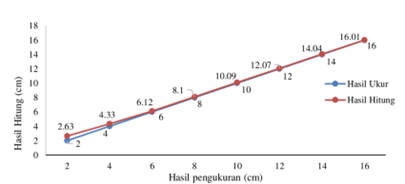
\includegraphics[width=0.75\textwidth]{gambar_hasil1.png}
  \caption{Contoh gambar hasil eksperimen 1}
  \label{fig:hasil1}
\end{figure}

% Setiap gambar harus dirujuk dan dibahas dalam paragraf
Grafik pada Gambar~\ref{fig:hasil1} menunjukkan hubungan antara pengukuran dan
perhitungan dari Persamaan~\ref{eq:linear}.

\begin{figure}[H]
  \centering
  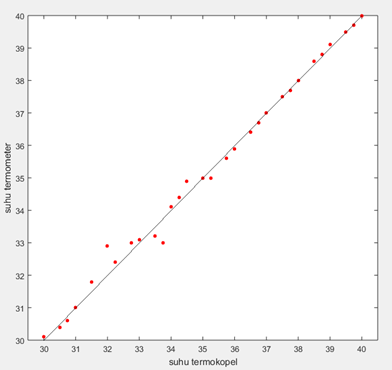
\includegraphics[width=0.75\textwidth]{gambar_hasil2.png}
  \caption{Contoh gambar hasil eksperimen 2 dengan nama gambar yang cukup panjang
  sehingga diperlukan penataan yang baik dalam daftar gambar}
  \label{fig:hasil2}
\end{figure}

Grafik pada Gambar~\ref{fig:hasil2} menunjukkan hubungan antara sensor suhu 1 dan
sensor suhu 2 yang dibentuk dari Persamaan~\ref{eq:gradien}.